\claude{
\section{Forecast selection and sampled-query estimation}\label{app:forecast_utility}
We train recurrent networks to produce the oscillations in Table~\ref{tab:generator_phases} and also record an untrained network. For each record, we use the observed segment of one neuron's activity to select and fit a model that predicts the next samples.

\begin{table}[htbp]
\centering\small
\caption{Forecast benchmark design. Network sizes are in Table~\ref{tab:architectures}.}
\label{tab:forecast-design}
\begin{tabularx}{\linewidth}{@{}p{.25\linewidth}X@{}}
\toprule
Component & Setting \\
\midrule
Trained dynamics & FORCE with RLS, gain 1.2, integration step 0.1, 40,000 steps. The RLS matrix starts at identity and updates every 2 steps. \\
Untrained network & Recurrent gain 1.5. Depending on initialization, the network can settle to a constant state or remain time-varying. \\
Recorded activity & $\tanh(h_{t,2})$ (zero-based neuron 2). Discard 5,000 initial steps and record 8,192 samples. \\
Observed and later samples & Samples 4,096--6,143 and 6,144--6,175, respectively \\
Fixed forecasts & Repeat the last value, the mean of the observed samples, or the values from 314 steps earlier. \\
Fitted forecasts & Ridge and 5-nearest-neighbor regression at lags 8 and 48; ridge on 64 random Fourier features at lag 48 \\
Forecast parameters & Ridge penalty 1, intercept penalty $10^{-8}$, Fourier bandwidth $1/48$. Clip standardized forecasts at $\pm10$. \\
Near-constant observations & Repeat the last value if the observed standard deviation is below $10^{-10}$. In NMSE, use observed variance or $10^{-12}$, whichever is larger. \\
Training the selection rule & 18 repeats and three validation folds grouped by initialization. Decision trees have maximum depth 2 or 3 and at least 8 examples per leaf. Random forests use 100 trees of depth at most 3 or 6 and at least 5 examples per leaf. \\
Held-out model search & Fit each candidate to four initial segments of increasing length. Test each fit on the next 32 observed samples. Choose the model with the lowest mean error and refit it on all observed samples. \\
Query budgets & Main budget 128; sensitivity checks at 64 and 256; blocks of 64 queries \\
Timing & Intel Core i5-12500H, one numerical thread. Use the same 12 inputs for every rule. After an untimed run, repeat seven times per input, changing the order of the rules between repetitions. \\
\bottomrule
\end{tabularx}
\end{table}

The learned selection rules predict each candidate's error. Summary statistics of the observed segment are its mean, standard deviation, fitted slope, lag-one correlation, normalized squared changes between adjacent samples, minimum error when aligned with a shifted copy, spectral entropy, and the fraction of spectral power in the largest peak. The held-out error features give the validation error of each candidate. All learned rules use the same training procedure, with tasks from each initialization kept in the same fold. We estimate replacements for missing features from the training portion of each fold.

\begin{table}[ht]
\centering\small
\caption{Forecast NMSE across model-selection rules. Entries show mean $\pm$ standard deviation.}
\label{tab:forecast_all}
\begin{tabular}{lrr}
\toprule
Selector & \cx{Full-query test ($n=30$)} & \cx{Query sampling test ($n=20$)} \\
\midrule
MG & $0.03138\,\cx{\pm 0.02369}$ & $0.03637\,\cx{\pm 0.02128}$ \\
Best fixed on development runs & $0.04475\,\cx{\pm 0.02978}$ & $0.06041\,\cx{\pm 0.05629}$ \\
Held-out model search & $0.03224\,\cx{\pm 0.03094}$ & $0.04074\,\cx{\pm 0.03236}$ \\
Cheap features & $0.04517\,\cx{\pm 0.02836}$ & $0.05923\,\cx{\pm 0.04999}$ \\
Cheap + held-out search & $0.03617\,\cx{\pm 0.02199}$ & $0.03379\,\cx{\pm 0.01753}$ \\
Held-out errors & $0.03997\,\cx{\pm 0.02869}$ & $0.03424\,\cx{\pm 0.02069}$ \\
Held-out errors + MG & $0.03423\,\cx{\pm 0.02164}$ & $0.03167\,\cx{\pm 0.02162}$ \\
Cheap + MG & $0.03138\,\cx{\pm 0.02369}$ & $0.03637\,\cx{\pm 0.02128}$ \\
Cheap + held-out search + MG & $0.03534\,\cx{\pm 0.02528}$ & $0.03994\,\cx{\pm 0.02952}$ \\
TwoNN & $0.03540\,\cx{\pm 0.02669}$ & $0.04364\,\cx{\pm 0.02027}$ \\
Levina--Bickel & $0.04054\,\cx{\pm 0.03208}$ & $0.04732\,\cx{\pm 0.04060}$ \\
Delay covariance PR & $0.04397\,\cx{\pm 0.02700}$ & $0.06098\,\cx{\pm 0.04815}$ \\
Permutation entropy & $0.04484\,\cx{\pm 0.03033}$ & $0.05384\,\cx{\pm 0.05040}$ \\
Sample entropy & $0.04718\,\cx{\pm 0.03284}$ & $0.05954\,\cx{\pm 0.04444}$ \\
All features except MG & $0.03669\,\cx{\pm 0.02740}$ & $0.03939\,\cx{\pm 0.02625}$ \\
All features including MG & $0.03420\,\cx{\pm 0.02191}$ & $0.04071\,\cx{\pm 0.02865}$ \\
Oracle (future targets) & $0.00759\,\cx{\pm 0.00622}$ & $0.00847\,\cx{\pm 0.00741}$ \\
\addlinespace
\cx{Paired improvement over search (95\% CI)}
 & \cx{$[-0.0102,\,0.0125]$}
 & \cx{$[-0.0073,\,0.0176]$} \\
\bottomrule
\end{tabular}

\end{table}

We average tasks within each repeat. The interval in Table~\ref{tab:forecast_all} resamples the within-repeat error differences between search and MG. Choosing from the measured continuation gives the lowest error attainable by the candidate set.

\paragraph{Sampled-query MG.}
To reduce computation, we search for neighbors around $q$ evenly spaced query vectors. All $n$ delay vectors remain available as neighbors, subject to the same time exclusion. The zero-based query indices are \cx{$\lfloor \ell(n-1)/(q-1)\rfloor$ for $\ell=0,\ldots,q-1$}, with $2\le q\le n$. For the selected set $Q$, we compute
\begin{equation}
\widehat d_{\rm MG}^{(q)}=
\frac{q(k-1)-1}{\displaystyle\sum_{i\in Q}\sum_{j=1}^{k-1}\log(r_{ik}/r_{ij})}.
\label{eq:querymg}
\end{equation}
\cx{When $Q$ contains every query and passes the numerical checks, the formula reduces to Equation~\eqref{eq:mg}.} We check the selected distances and sums against the numerical limits. Insufficient neighbors, nonfinite values, or constant records yield unavailable estimates. The model-selection rule uses the replacements learned on development runs for missing scores.

\cx{The blocked implementation computes distances to all vectors for one block of queries at a time, at cost $O(qnE)$ for the distance calculations. The full implementation uses a KD-tree. Table~\ref{tab:forecast_utility} compares the two implementations as used.}

\paragraph{Timing on the same inputs.}
Timing includes computing features, choosing a forecaster, and fitting it. All three timed rules use the same inputs. For each input we take the median time over repetitions, then report the median across inputs (Table~\ref{tab:forecast_utility}).


\section{Comparing intervention rules}\label{app:intervention_utility}
Stopping early can limit memorization of noisy labels. Freezing layers or pruning hidden neurons can reduce the computation needed for later updates. We compare when MG-based rules, simpler statistics, and fixed schedules intervene. All rules use the same development runs and candidate times.

For the stopping experiments, we replace some training labels with randomly chosen incorrect labels. The freezing and pruning experiments retain the original training labels. The rules use weight norm or loss on a fixed set of training images with their assigned labels (Table~\ref{tab:mnist-intervention-setup}).

\begin{table}[htbp]
\centering\small
\caption{MNIST intervention protocol.}
\label{tab:mnist-intervention-setup}
\begin{tabularx}{\linewidth}{@{}p{.30\linewidth}X@{}}
\toprule
Component & Setting \\
\midrule
Data & $14\times14$ images after pooling. Use 2,000 for training, 500 for validation, and 2,000 for testing. Validation and test labels are unchanged. \\
Training & Adam at $10^{-3}$, batch 64, at most 2,048 updates \\
Label corruption & 40\% or 60\%; wrong classes sampled independently for each run \\
Fixed set for loss & 128 training examples, using their assigned labels \\
Candidate updates & 256, 512, 768, 1,024, 1,536 \\
Repeats & Use 3 repeats to choose the rule and 8 separate repeats to evaluate it. \\
Pruned layers & Retain 64 neurons per hidden layer. Rank neurons by the product of the norms of their incoming and outgoing weights. \\
\bottomrule
\end{tabularx}
\end{table}

The scalar rules use completed windows. A rule based on the window mean compares it with a threshold. A fixed schedule chooses the same step in every evaluation run. Training runs to the full budget if the rule never triggers.

We score each rule by validation accuracy with a penalty for computation. We maximize $A-0.02C$, where $A$ is mean validation accuracy as a fraction and $C$ is the mean number of estimated multiply--accumulate operations relative to uninterrupted training. Saving half the operations improves this score as much as one percentage point of accuracy.

\begin{figure}[htbp]
\centering
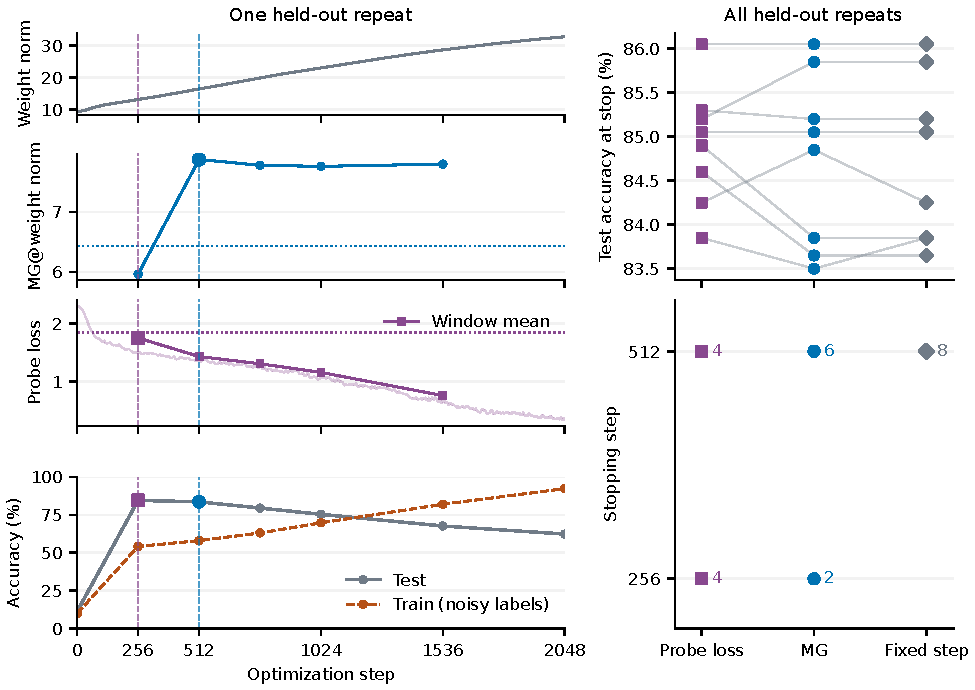
\includegraphics[width=.96\linewidth]{figures/mnist_stop_trace.pdf}
\caption{Early stopping on MNIST with 40\% noisy labels. Left, thresholds and stopping steps in one run. Right, within-run differences in test accuracy and counts of stops by step.}
\label{fig:mnist-stop-trace}
\end{figure}

The MG and fixed-set loss rules can stop at different training steps with similar test accuracy across repeats (Figure~\ref{fig:mnist-stop-trace}).

Freezing holds the hidden-layer weights fixed and continues training the classifier. Pruning removes hidden neurons and keeps the retained weights and their optimizer state. After intervention, both runs use the same minibatches as uninterrupted training.

\begin{table*}[ht]
\centering\small
\caption{MNIST test accuracy (\%) and relative arithmetic cost across eight repeats.}
\label{tab:intervention_utility}
\begin{tabular}{@{}l*{4}{rr}@{}}
\toprule
 & \multicolumn{2}{c}{Stop, 40\% noise} & \multicolumn{2}{c}{Stop, 60\% noise} & \multicolumn{2}{c}{Freeze} & \multicolumn{2}{c}{Prune} \\
\cmidrule(lr){2-3}\cmidrule(lr){4-5}\cmidrule(lr){6-7}\cmidrule(lr){8-9}
Rule & Acc. & Cost & Acc. & Cost & Acc. & Cost & Acc. & Cost \\
\midrule
MG & 84.75 & 0.219 & 76.58 & 0.125 & 91.53 & 0.535 & 92.44 & 0.572 \\
Window mean & 84.90 & 0.188 & 76.58 & 0.125 & 91.32 & 0.515 & 92.50 & 0.618 \\
Spectral entropy & 84.67 & 0.203 & 76.58 & 0.125 & 91.32 & 0.515 & 92.38 & 0.553 \\
Fixed schedule & 84.72 & 0.250 & 76.58 & 0.125 & 91.32 & 0.515 & 92.52 & 0.628 \\
Uninterrupted training & 64.11 & 1.000 & 43.83 & 1.000 & 92.29 & 1.000 & 92.29 & 1.000 \\
\bottomrule
\end{tabular}

\end{table*}

Early stopping improves test accuracy when some training labels are incorrect. Pruning preserves accuracy while reducing the estimated number of operations. Simple rules often match MG (Table~\ref{tab:intervention_utility}).
}
